\documentclass[11pt,a4paper]{article}

\usepackage[T1]{fontenc}
\usepackage[utf8]{inputenc}
\usepackage{lmodern}
\usepackage{microtype}
\usepackage[a4paper,margin=2.45cm]{geometry}
\usepackage{amsmath,amssymb}
\usepackage{booktabs,array}
\usepackage{xcolor}
\usepackage{graphicx}
\usepackage[hidelinks]{hyperref}
\usepackage{tikz}
\usetikzlibrary{positioning,arrows.meta,shapes.geometric}

\setlength{\parindent}{1.4em}
\setlength{\parskip}{0.15em}
\setlength{\emergencystretch}{2em}
\newcolumntype{P}[1]{>{\raggedright\arraybackslash}p{#1}}

% Replace a placeholder with \includegraphics[width=\linewidth]{figures/name.pdf}
% when the final publication figure has been generated.
\newcommand{\plotplaceholder}[2]{%
\fbox{\begin{minipage}[c][#1][c]{0.92\linewidth}
\centering\color{gray!70}\large\textbf{Figure placeholder}\\[0.5em]
\normalsize #2
\end{minipage}}}
\newcommand{\figsource}[1]{\par\smallskip\textit{Figure source: #1}}

\title{From Random Packing to an Interpretable Transport Closure:\\
Structure-Resolved CO$_2$ Adsorption in DEM-Generated Zeolite Beds}
\author{Ali Khalifa$^{1}$ and .... $^{2}$\\[0.4em]
\small $^{1}$Technical University of Munich, Freising, Germany}
\date{}

\begin{document}
\maketitle

\begin{abstract}
Packed beds with almost the same porosity can contain different connected void
pathways. These differences may change how quickly carbon dioxide reaches and
uses the adsorbent, but they are hidden by conventional bulk descriptors. We
study this effect without computational fluid dynamics. Twenty beds containing
1850 spherical commercial zeolite 13X beads were generated by the discrete-
element method. Their void spaces were converted into pore networks, on which a
conservative diffusion--adsorption model was solved. Gas diffusion through pore
throats was coupled to one linear-driving-force adsorption equation per bead.
Only the random packing realization changed between cases. The robust bulk
porosity varied by about 0.55\%, whereas CO$_2$ uptake at 5000~s varied by
11.0\%. A homogeneous one-dimensional model reproduced the network uptake
curves with a mean time-weighted normalized error of 1.58\%, but its fitted
effective diffusivity varied by 23.1\%. Porosity could not predict this
coefficient in leave-one-bed-out tests ($R^2=-0.234$). In contrast, an
inlet-to-interior pore-network conductance produced an accessibility
diffusivity that correlated strongly with the fitted coefficient. A positive
power-law closure predicted withheld beds with $R^2=0.890$. The results show
that connectivity and entrance accessibility contain transport information
that is absent from bulk porosity. The framework provides an interpretable
bridge from particle-resolved geometry to a cheap homogeneous adsorption
model, while keeping adsorption thermodynamics and mass conservation explicit.
\end{abstract}

\noindent\textbf{Keywords:} CO$_2$ capture; zeolite 13X; packed bed; DEM;
pore network; adsorption; effective diffusivity; physical closure

\section{Introduction}

Packed beds of porous particles are widely used for gas separation and CO$_2$
capture. Their performance depends on two different scales. At the particle
scale, the adsorbent material determines equilibrium capacity and uptake rate.
At the bed scale, the arrangement of particles determines the empty pathways
through which gas reaches the adsorbent. Standard one-dimensional models
usually represent this second scale using porosity and one effective transport
coefficient. This is efficient, but porosity alone does not describe whether
the void space is well connected or contains entrance bottlenecks.

Particle-resolved computational fluid dynamics could examine these pathways,
but it is expensive for an ensemble of stochastic beds. Here we use a simpler
physics-based route. The discrete-element method (DEM) creates mechanically
realistic particle arrangements. A pore network extracted from each packing
then represents the void space as connected pore bodies and throats
\cite{Blunt2017}. CO$_2$ diffusion is solved on this network and coupled to
adsorption by every zeolite bead.

The goal is not to reproduce a flowing industrial adsorption column. The bed
contains stagnant gas, and CO$_2$ enters by diffusion from a reservoir at the
bottom. This restricted problem isolates the effect of packing structure. It
allows us to ask a precise question: can a simple, measurable property of the
pore network explain packing-to-packing changes that bulk porosity misses?

The main contribution is an interpretable closure linking a geometry-derived
accessibility conductance to the effective diffusivity of a homogeneous
one-dimensional adsorption model. The study deliberately uses simple physical
descriptors rather than a graph neural network because only twenty independent
packings are presently available.

\section{Physical problem and modelling workflow}

The bed initially contains nitrogen with zero CO$_2$ concentration and the
zeolite beads initially contain no adsorbed CO$_2$. The lower boundary is
connected to a reservoir at $c_{\mathrm{in}}=6.05$~mol~m$^{-3}$. The top and
cylindrical wall are closed. Temperature is constant at 298.15~K. There is no
imposed velocity, pressure-drop calculation, heat of adsorption or CFD.

Figure~\ref{fig:problem} illustrates the model. Large circles represent
zeolite beads. Small blue nodes and connecting lines represent the pore network.
Gas diffuses through this network and is adsorbed by adjacent particles.

\begin{figure}[!htbp]
\centering
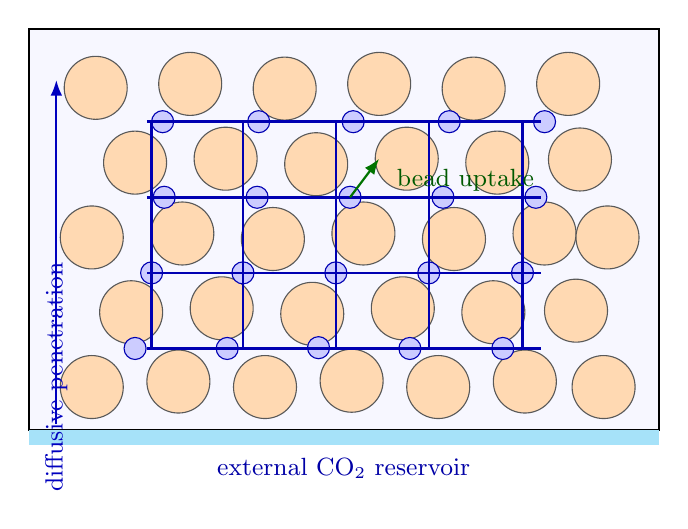
\begin{tikzpicture}[
 bead/.style={circle,draw=black!65,fill=orange!30,minimum size=8mm},
 pore/.style={circle,draw=blue!70!black,fill=blue!20,minimum size=2.8mm,inner sep=0pt},
 throat/.style={draw=blue!70!black,line width=0.9pt},
 arr/.style={-{Latex[length=2mm]},thick},font=\small]
\fill[blue!3] (0,0) rectangle (8,5.1);
\draw[thick] (0,0) rectangle (8,5.1);
\fill[cyan!35] (0,-0.18) rectangle (8,0);
\node[blue!65!black] at (4,-0.48) {external CO$_2$ reservoir};
\foreach \x/\y in {0.8/0.55,1.9/0.62,3.0/0.55,4.1/0.63,5.2/0.55,6.3/0.62,7.3/0.55,
1.3/1.50,2.45/1.55,3.6/1.48,4.75/1.55,5.9/1.50,6.95/1.52,
0.8/2.45,1.95/2.50,3.1/2.43,4.25/2.50,5.4/2.43,6.55/2.50,7.35/2.45,
1.35/3.40,2.5/3.45,3.65/3.38,4.8/3.45,5.95/3.40,7.0/3.44,
0.85/4.35,2.05/4.40,3.25/4.34,4.45/4.40,5.65/4.34,6.85/4.40}
\node[bead] at (\x,\y) {};
\foreach \x/\y in {1.35/1.04,2.52/1.04,3.68/1.05,4.84/1.04,6.02/1.04,
1.56/2.00,2.72/2.00,3.90/2.00,5.08/2.00,6.27/2.00,
1.72/2.96,2.90/2.96,4.08/2.96,5.26/2.96,6.44/2.96,
1.70/3.92,2.92/3.92,4.12/3.92,5.34/3.92,6.55/3.92}
\node[pore] at (\x,\y) {};
\foreach \ya/\yb in {1.04/2.00,2.00/2.96,2.96/3.92}
 \foreach \x in {1.56,2.72,3.90,5.08,6.27} \draw[throat] (\x,\ya)--(\x,\yb);
\foreach \y in {1.04,2.00,2.96,3.92}
 \draw[throat] (1.5,\y)--(6.5,\y);
\draw[arr,blue!75!black] (0.35,0.08)--(0.35,4.45)
 node[midway,left,rotate=90]{diffusive penetration};
\draw[arr,green!45!black] (4.08,2.96)--(4.45,3.45);
\node[anchor=west,green!35!black] at (4.55,3.18) {bead uptake};
\end{tikzpicture}
\caption{Schematic of the diffusion--adsorption problem. DEM supplies the
particle positions. A geometry-derived pore graph carries gas-phase CO$_2$,
and each particle has its own adsorbed loading. This vector schematic is drawn
directly in this TeX file and needs no external data.}
\label{fig:problem}
\end{figure}

The complete workflow is shown in Fig.~\ref{fig:workflow}. DEM and the pore
network provide the detailed reference model. The homogeneous model is the
cheap reduced description. The closure connects them.

\begin{figure}[!htbp]
\centering
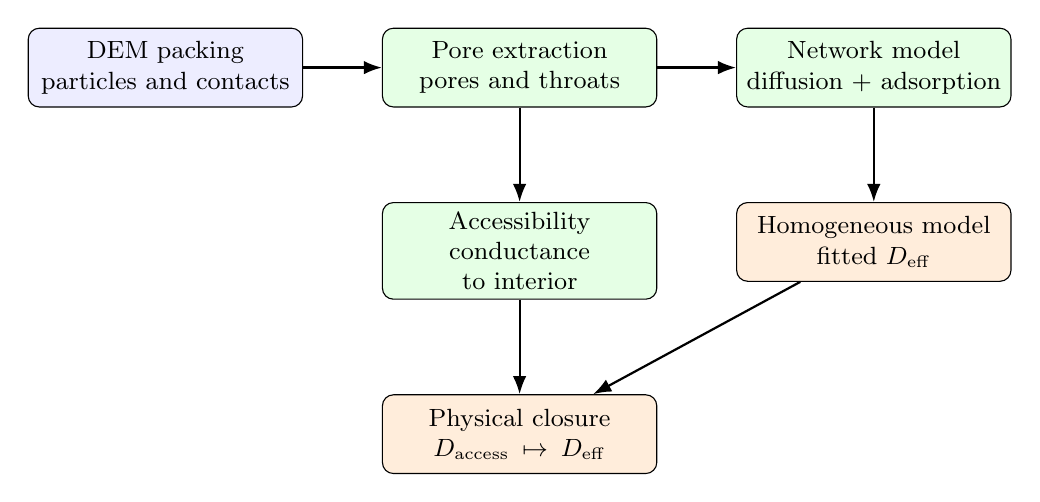
\begin{tikzpicture}[
 box/.style={draw,rounded corners,align=center,text width=3.25cm,minimum height=1.0cm,fill=blue!7},
 phys/.style={box,fill=green!10}, reduced/.style={box,fill=orange!14},
 arr/.style={-{Latex[length=2.3mm]},thick},font=\small]
\node[box] (dem) {DEM packing\\particles and contacts};
\node[phys,right=1.0cm of dem] (net) {Pore extraction\\pores and throats};
\node[phys,right=1.0cm of net] (ads) {Network model\\diffusion + adsorption};
\node[phys,below=1.2cm of net] (acc) {Accessibility\\conductance to interior};
\node[reduced,below=1.2cm of ads] (hom) {Homogeneous model\\fitted $D_{\mathrm{eff}}$};
\node[reduced,below=1.2cm of acc] (closure) {Physical closure\\$D_{\mathrm{access}}\mapsto D_{\mathrm{eff}}$};
\draw[arr] (dem)--(net); \draw[arr] (net)--(ads);
\draw[arr] (net)--(acc); \draw[arr] (ads)--(hom);
\draw[arr] (acc)--(closure); \draw[arr] (hom)--(closure);
\end{tikzpicture}
\caption{Physics-focused hybrid workflow. The pore network generates detailed,
conservative adsorption curves, while the homogeneous model provides the cheap
description used at larger scales. This vector diagram is contained in the
TeX source.}
\label{fig:workflow}
\end{figure}

\section{Methods}

\subsection{DEM packing ensemble}

Twenty independent cylindrical beds were generated with LAMMPS. Every bed
contains 1850 monodisperse spheres of diameter 1.6~mm and apparent density
1600~kg~m$^{-3}$. The tube diameter is 16~mm, giving
$D_{\mathrm{tube}}/d_p=10$. Gravity, Hertz--Mindlin contacts, friction and
damping were used to fill and settle the beds. Only the insertion seed changed.
A packing was accepted only if it contained all particles, was mechanically
settled and passed overlap and geometry checks.

Bulk porosity was calculated using a robust bed top defined by the 99th
percentile of particle-top elevations. Sphere intersections with axial and
radial bins were integrated instead of assigning each complete sphere to one
bin. This prevents artificial jumps in local porosity.

\begin{figure}[!htbp]
\centering
\plotplaceholder{6.2cm}{ParaView rendering of three representative DEM beds,
preferably the lowest-, median- and highest-accessibility realizations. Show
the same camera, tube outline and bead size in all panels.}
\caption{Representative DEM-generated zeolite beds. The final figure should
show that all cases have the same particle and tube sizes but differ slightly
in local arrangement. \figsource{Open the particle VTP files in
\texttt{paraview\_co2\_packings/seed\_*/particles\_final.vtp}. If seed
subfolders were not retained, regenerate them from
\texttt{co2\_13x\_seed\_*/particles\_final.dump} using
\texttt{convert\_co2\_packings\_to\_vtp.py}.}}
\label{fig:packings}
\end{figure}

\subsection{Pore-network extraction}

The void geometry was converted to a Delaunay--Voronoi pore network. A pore
body stores gas volume and concentration. Two pore bodies are connected by a
throat when their Delaunay tetrahedra share a face. For a throat connecting
pores $i$ and $j$, the diffusive conductance is
\begin{equation}
 G_{ij}=D_m\frac{A_{ij}}{L_{ij}},
 \label{eq:throat}
\end{equation}
where $D_m=1.5\times10^{-5}$~m$^2$~s$^{-1}$, $A_{ij}$ is the open throat area
and $L_{ij}$ is its length. Pore volumes were allocated using
$2^{22}=4{,}194{,}304$ Sobol samples. All networks were connected, spanned the
bed and conserved total void volume. For example, seed 18427 contained 9397
pores and 18104 throats.

\begin{figure}[!htbp]
\centering
\plotplaceholder{6.4cm}{ParaView overlay of zeolite particles and the extracted
pore network for seed 18427. Use spheres for particles, points for pore bodies
and lines for throats; include a magnified inset near the inlet.}
\caption{Particle packing and corresponding pore network for the verification
case. The overlay provides a direct geometric check that pore nodes occupy the
void space and throats connect neighboring void regions. \figsource{Use
\texttt{paraview\_co2\_packings/.../particles\_final.vtp} together with
\texttt{co2\_pore\_networks\_power22/seed\_18427/pore\_network.vtp}. The
underlying tables are \texttt{pores.csv} and \texttt{throats.csv} in the same
network directory.}}
\label{fig:network}
\end{figure}

\subsection{Conservative diffusion--adsorption model}

Each pore $i$ has gas concentration $c_i$ and volume $V_i$. Each zeolite bead
$k$ has mean adsorbed loading $q_k$ in mol~kg$^{-1}$. The gas balance is
\begin{equation}
 V_i\frac{dc_i}{dt}=\sum_jG_{ij}(c_j-c_i)
 -\sum_k w_{ki}m_k\frac{dq_k}{dt}.
 \label{eq:porebalance}
\end{equation}
The weights $w_{ki}$ distribute bead uptake among adjacent pores and sum to one
for each bead. Therefore, every mole removed from the gas is added to the
solid.

Equilibrium loading is represented by the Langmuir form
\begin{equation}
 q_k^*=\frac{q_sbp_k}{1+bp_k},\qquad p_k=c_k^gRT,
 \label{eq:langmuir}
\end{equation}
and bead uptake follows the linear-driving-force equation
\begin{equation}
 \frac{dq_k}{dt}=k_{\mathrm{LDF}}(q_k^*-q_k).
 \label{eq:ldf}
\end{equation}
The adopted parameters are $q_s=5.332$~mol~kg$^{-1}$,
$b=5.093\times10^{-5}$~Pa$^{-1}$ and
$k_{\mathrm{LDF}}=8.55\times10^{-3}$~s$^{-1}$. The affinity assumes that a
published table omitted a factor of $10^{-3}$; this assumption is discussed in
Sec.~\ref{sec:limitations}. The kinetic coefficient is inferred from the
commercial 13X bead time constant reported by Hu et al.~\cite{Hu2014}.

At the inlet, every labelled inlet pore is connected to the same external
reservoir. The nominal areas assigned to these connections sum to the full tube
cross-section, $A_{\mathrm{tube}}=\pi R^2$. Internal blockage remains represented
by the pore and throat geometry. The stiff coupled equations were integrated
with an implicit BDF method and an analytical sparse Jacobian.

\subsection{Accessibility descriptor}

The main structural descriptor is a steady conductance from the inlet to a
plane $5d_p$ inside the bed. Inlet-pore concentration is set to one and the
interior-plane concentration to zero. Conservation is solved in all pores
between them. The resulting total flux is the effective accessibility
conductance $G_{\mathrm{access}}$. It is converted to diffusivity units by
\begin{equation}
 D_{\mathrm{access}}=
 \frac{G_{\mathrm{access}}H}{A_{\mathrm{tube}}}.
 \label{eq:daccess}
\end{equation}
The same calculation was repeated at $3d_p$, $7d_p$ and $10d_p$ to check that
the conclusion did not depend on one analysis plane.

\subsection{Homogeneous one-dimensional model}

The reduced model divides the bed height into 100 finite-volume cells. It does
not contain individual pores or particles:
\begin{align}
 \varepsilon_b\frac{\partial c}{\partial t}
 &=D_{\mathrm{eff}}\frac{\partial^2c}{\partial z^2}
 -(1-\varepsilon_b)\rho_p\frac{\partial q}{\partial t},
 \label{eq:homgas}\\
 \frac{\partial q}{\partial t}&=k_{\mathrm{LDF}}[q^*(c)-q].
 \label{eq:homads}
\end{align}
The isotherm, kinetic coefficient, inlet concentration, bed height and initial
conditions are the same as in the network model. Only $D_{\mathrm{eff}}$ is
fitted for each bed. The inlet uses a Robin condition that includes both the
external resistance and diffusion across half of the first numerical cell.
The fit minimizes a time-integrated squared uptake error.

\subsection{Statistical analysis and closure}

Predictive tests leave out one complete bed, fit the model to the remaining 19
beds and predict the omitted bed. This is repeated twenty times. We report the
resulting $R^2$, RMSE and mean absolute percentage error. Parameter uncertainty
is estimated by 10,000 bed-level bootstrap samples. Target permutation tests
use 5000 random permutations.

Three useful closure forms are compared:
\begin{align}
 D_{\mathrm{eff}}&=a_0+a_1\varepsilon_b,\\
 D_{\mathrm{eff}}&=\alpha D_{\mathrm{access}},\\
 D_{\mathrm{eff}}&=C D_{\mathrm{access}}^n.
\end{align}
Affine conductance models are also evaluated as numerical baselines. The power
law is reported in normalized form so that its coefficient is dimensionless.

\section{Results}

\subsection{Matched porosity but different adsorption response}

All twenty packings passed mechanical and pore-network quality checks. Mean
robust bulk porosity was 0.44665 and its coefficient of variation was about
0.55\%. The mean bed height was 35.61~mm. Despite this close global matching,
uptake at 5000~s ranged from 0.2056 to 0.3148~mol~kg$^{-1}$, with a coefficient
of variation of 11.04\%. The mean relative half-uptake time was 1501~s.

\begin{figure}[!htbp]
\centering
\plotplaceholder{6.3cm}{Two-panel plot: (a) robust bulk and interior porosity
for all 20 seeds; (b) mean uptake curves for all 20 pore-network simulations,
with one highlighted low-, median- and high-uptake case.}
\caption{Global packing similarity and transient response variability. Panel
(a) should demonstrate the narrow porosity range, whereas panel (b) should show
that the adsorption curves remain meaningfully different. \figsource{Porosity
data and existing profiles are in \texttt{co2\_porosity\_analysis/}. Uptake
curves are in
\texttt{co2\_adsorption\_campaign\_finite\_inlet\_5000s/seed\_*/timeseries.csv};
campaign values are in
\texttt{co2\_adsorption\_finite\_inlet\_analysis/co2\_adsorption\_campaign\_dataset.csv}.}}
\label{fig:campaign}
\end{figure}

\subsection{Spatially heterogeneous utilization}

The bed remained far from equilibrium at 5000~s. For seed 18427, mean loading
was 0.2843~mol~kg$^{-1}$, only about 12.3\% of the equilibrium loading at the
inlet concentration. CO$_2$ entered from below, so lower particles were used
more strongly than particles deeper in the bed. Particle-loading coefficients
of variation ranged from 1.79 to 2.03 across the ensemble.

\begin{figure}[!htbp]
\centering
\plotplaceholder{6.4cm}{ParaView particle-loading maps at selected times,
for example 100, 1000 and 5000 s, or a final comparison of low- and
high-accessibility beds. Use the same color scale in every panel.}
\caption{Spatial development of particle loading. A common color range is
essential so that penetration and underutilized regions can be compared
directly. \figsource{Particle coordinates are in
\texttt{co2\_13x\_seed\_*/particles\_final.dump}. Particle loadings are in
\texttt{co2\_adsorption\_campaign\_finite\_inlet\_5000s/seed\_*/final\_state.npz}.
Use the pore-network \texttt{particle\_pore\_incidence.csv} if mapping support
is needed. A publication-figure script can write the combined VTP files.}}
\label{fig:loadingmap}
\end{figure}

\subsection{Accessibility explains transient utilization}

The inlet-to-interior conductance correlates with uptake at 5000~s with
Spearman $\rho=0.968$. It correlates negatively with the underutilized-particle
fraction ($\rho=-0.959$). The unique number of second-layer pores correlates
with half-uptake time ($\rho=-0.814$). Porosity-only leave-one-bed-out models
give negative $R^2$ values for these responses. Conductance alone predicts
uptake with $R^2=0.924$ and the underutilized fraction with $R^2=0.863$.

\begin{figure}[!htbp]
\centering
\plotplaceholder{6.2cm}{Three scatter plots with seed labels or selected labels:
(a) porosity versus uptake, (b) inlet-to-interior conductance versus uptake,
and (c) conductance versus underutilized-particle fraction. Include bootstrap
trend intervals and report Spearman correlation in each panel.}
\caption{Why bulk porosity is insufficient. The figure should contrast the
absence of a useful porosity trend with the strong accessibility relationships.
\figsource{Use
\texttt{co2\_adsorption\_finite\_inlet\_analysis/co2\_adsorption\_campaign\_dataset.csv},
the merged structure table produced by
\texttt{extract\_co2\_inlet\_accessibility.py}, and statistical outputs in
\texttt{co2\_reduced\_physical\_model\_analysis/}.}}
\label{fig:accessresponses}
\end{figure}

\subsection{Homogeneous reduction}

The 100-cell homogeneous model fitted all twenty network curves successfully.
The mean time-weighted normalized RMSE was 1.58\%, with a range from 0.84 to
2.46\%. Fitted $D_{\mathrm{eff}}$ ranged from
$4.340\times10^{-7}$ to $1.096\times10^{-6}$~m$^2$~s$^{-1}$, giving a
coefficient of variation of 23.13\%. Thus, the homogeneous model is accurate,
but its transport coefficient must retain packing-specific information.

A 100--200--400-cell comparison for seed 18427 changed $D_{\mathrm{eff}}$ by
0.156\% and then 0.039\%, supporting the 100-cell choice. The maximum absolute
mass-balance residual in the accepted test was $1.38\times10^{-13}$~mol.

\begin{figure}[!htbp]
\centering
\plotplaceholder{6.2cm}{Two panels: (a) pore-network and best-fit homogeneous
uptake curves for representative low-, median- and high-diffusivity beds;
(b) residual or relative-error curves.}
\caption{Accuracy of the one-dimensional homogeneous reduction. Curves should
be evaluated over the full 0--5000~s interval, not only at the final time.
\figsource{Network curves are in
\texttt{co2\_adsorption\_campaign\_finite\_inlet\_5000s/seed\_*/timeseries.csv}.
Homogeneous curves and fit comparisons are in
\texttt{co2\_homogeneous\_campaign\_100cells/seed\_*/timeseries.csv} and
\texttt{fit\_comparison.csv}; campaign parameters are in
\texttt{co2\_homogeneous\_campaign\_100cells/homogeneous\_campaign\_summary.csv}.}}
\label{fig:homfits}
\end{figure}

\subsection{Effective-diffusivity closure}

At $5d_p$, $D_{\mathrm{access}}$ and fitted $D_{\mathrm{eff}}$ have Pearson
correlation 0.951 and Spearman correlation 0.953. A porosity-only model gives
leave-one-bed-out $R^2=-0.234$. A direct proportional closure,
$D_{\mathrm{eff}}=\alpha D_{\mathrm{access}}$, gives
$\alpha=0.1523$ with bootstrap interval 0.1427--0.1616, but its predictive
$R^2$ is only 0.555. It is therefore too restrictive.

The affine accessibility model reaches $R^2=0.881$, but its negative intercept
can produce negative diffusivity outside the fitted range. The positive power
law gives almost the same predictive accuracy without this problem:
\begin{equation}
 \boxed{\frac{D_{\mathrm{eff}}}{D_m}=0.7589
 \left(\frac{D_{\mathrm{access}}}{D_m}\right)^{2.4969}}.
 \label{eq:closure}
\end{equation}
Its leave-one-bed-out $R^2$ is 0.890. The bootstrap median exponent is 2.504
with a 95\% interval of 2.057--2.768. The raw-conductance affine model gives a
slightly higher $R^2=0.898$, but also has a negative intercept and is less
portable because it does not account for bed height and area.

\begin{figure}[!htbp]
\centering
\plotplaceholder{6.2cm}{Two panels: (a) fitted effective diffusivity versus
accessibility diffusivity, showing the positive power-law curve and bootstrap
band; (b) observed versus leave-one-bed-out predicted diffusivity for the
porosity, proportional and power-law models.}
\caption{Formal closure from pore-network accessibility to homogeneous
effective diffusivity. The one-to-one line in panel (b) should be shown.
\figsource{All required joined values are in
\texttt{co2\_effective\_diffusivity\_closure/closure\_dataset.csv}. Use
\texttt{closure\_loo\_predictions.csv},
\texttt{closure\_bootstrap\_intervals.csv} and
\texttt{closure\_summary.json} in the same directory. Preliminary plots
\texttt{closure\_physical\_fit.*} and \texttt{closure\_loo\_predictions.*}
are also written there.}}
\label{fig:closure}
\end{figure}

\subsection{Sensitivity to the interior-plane depth}

Changing the interior plane from $3d_p$ to $10d_p$ reduces conductance because
the diffusion path becomes longer. Nevertheless, Pearson correlations with
$D_{\mathrm{eff}}$ remain between 0.936 and 0.951. Affine leave-one-bed-out
$R^2$ remains between 0.834 and 0.881. The result is therefore not caused by
the arbitrary choice of one plane. The $5d_p$ definition is retained because
it lies beyond the immediate inlet layer and gives the strongest prediction.

\begin{figure}[!htbp]
\centering
\plotplaceholder{5.8cm}{Depth-sensitivity plot showing correlation and
leave-one-bed-out R-squared at 3, 5, 7 and 10 particle diameters. A second axis
or panel may show the decrease in mean conductance with depth.}
\caption{Robustness to the definition of the inlet-accessibility depth.
\figsource{Use
\texttt{co2\_effective\_diffusivity\_closure/closure\_depth\_sensitivity.csv}
and the four input files
\texttt{co2\_inlet\_accessibility\_\{3,5,7,10\}dp.csv}.}}
\label{fig:depth}
\end{figure}

\section{Discussion}

The results separate three ideas that are often combined in one effective
parameter. First, porosity measures how much empty volume exists. Second,
connectivity determines whether this volume forms useful transport paths.
Third, entrance accessibility determines how easily CO$_2$ reaches those
paths from the boundary. The twenty beds have almost the same amount of void
space but different values of the latter two properties.

The homogeneous model shows that the detailed network curves can be reduced to
one packing-specific transport coefficient with small error. This is useful:
the pore network is needed to understand and construct the closure, but it does
not need to be solved whenever a larger-scale model uses the bed. Equation
\eqref{eq:closure} transfers the relevant geometric information into the cheap
one-dimensional model.

The power-law exponent is greater than one. Within the studied range, this
means that small improvements in inlet-to-interior accessibility accompany
larger relative improvements in fitted bed transport. This should be treated
as an empirical structural result, not yet as a universal law. The twenty beds
share one tube-to-particle ratio, bead size and material parameter set.

The study also illustrates why the statistically best equation is not always
the best physical closure. The raw-conductance affine model has a slightly
higher cross-validated $R^2$, but its negative intercept eventually predicts
negative diffusivity. The selected power law is always positive, is naturally
normalized and sacrifices little predictive accuracy.

\section{Limitations}\label{sec:limitations}

The model describes dry, isothermal, diffusion-driven filling from one side.
It does not describe pressure-driven breakthrough, pressure drop, heat release,
water competition or regeneration. The conclusions therefore concern the
influence of packing geometry on transient accessibility, not complete
industrial capture performance.

The adopted zeolite affinity $b=5.093\times10^{-5}$~Pa$^{-1}$ assumes that the
source table omitted a factor of $10^{-3}$. The LDF coefficient is converted
from a reported single-bead time constant at a somewhat higher temperature
\cite{Hu2014}. These values provide a documented and internally consistent
working case, but new material measurements would be needed for quantitative
prediction of a particular commercial batch.

Finally, all statistical observations come from twenty realizations of one
geometry. Leave-one-bed-out validation tests interpolation among these beds;
it does not test transfer to other particle sizes or tube-to-particle ratios.
Such external validation is a valuable later step but is outside the completed
scope reported here.

\section{Conclusions}

Twenty DEM-generated zeolite beds with closely matched porosity produced
meaningfully different transient CO$_2$ adsorption responses. A conservative
pore-network model traced these differences to inlet accessibility and internal
connectivity. A homogeneous one-dimensional model reproduced the detailed
uptake curves with a mean normalized error of 1.58\%, but required effective
diffusivities that varied by 23.1\% between beds.

Porosity could not predict this variation. A dimensionless positive power law
based on inlet-to-interior accessibility predicted withheld-bed effective
diffusivity with $R^2=0.890$. The work therefore provides a simple physical
message: equal void volume does not imply equal transport. How that void space
is connected to the inlet matters. The proposed closure preserves this
information in a form that can be used by a cheap homogeneous adsorption model
without CFD or a high-capacity machine-learning model.

\section*{Data and code availability}

The final publication package should contain the LAMMPS input, prescribed seed
list, packing-quality summary, pore-network extraction and QA scripts,
diffusion--adsorption solver, homogeneous fitting scripts, closure-analysis
script and the processed CSV tables identified in the figure captions. A
public repository DOI and archive link will be inserted here before submission.

\begin{thebibliography}{9}
\small

\bibitem{Blunt2017}
M.~J. Blunt,
\emph{Multiphase Flow in Permeable Media: A Pore-Scale Perspective}.
Cambridge University Press, 2017.

\bibitem{Dantas2011}
T.~L.~P. Dantas, F.~M.~T. Luna, I.~J. Silva Jr., A.~E.~B. Torres,
D.~C.~S. de Azevedo, A.~E. Rodrigues, and R.~F.~P. Moreira,
``Modeling of the fixed-bed adsorption of carbon dioxide and a carbon
dioxide--nitrogen mixture on zeolite 13X,''
\emph{Brazilian Journal of Chemical Engineering}, vol.~28, pp.~533--544, 2011.
\href{https://doi.org/10.1590/S0104-66322011000300018}{doi:10.1590/S0104-66322011000300018}.

\bibitem{Hu2014}
X.~Hu, E.~Mangano, D.~Friedrich, H.~Ahn, and S.~Brandani,
``Diffusion mechanism of CO$_2$ in 13X zeolite beads,''
\emph{Adsorption}, vol.~20, pp.~121--135, 2014.
\href{https://doi.org/10.1007/s10450-013-9554-z}{doi:10.1007/s10450-013-9554-z}.

\bibitem{Ruthven1984}
D.~M. Ruthven,
\emph{Principles of Adsorption and Adsorption Processes}.
Wiley, 1984.

\end{thebibliography}

\end{document}
